\documentclass[serif]{beamer}\usepackage[]{graphicx}\usepackage[]{color}
%% maxwidth is the original width if it is less than linewidth
%% otherwise use linewidth (to make sure the graphics do not exceed the margin)
\makeatletter
\def\maxwidth{ %
  \ifdim\Gin@nat@width>\linewidth
    \linewidth
  \else
    \Gin@nat@width
  \fi
}
\makeatother

\definecolor{fgcolor}{rgb}{0.345, 0.345, 0.345}
\newcommand{\hlnum}[1]{\textcolor[rgb]{0.686,0.059,0.569}{#1}}%
\newcommand{\hlstr}[1]{\textcolor[rgb]{0.192,0.494,0.8}{#1}}%
\newcommand{\hlcom}[1]{\textcolor[rgb]{0.678,0.584,0.686}{\textit{#1}}}%
\newcommand{\hlopt}[1]{\textcolor[rgb]{0,0,0}{#1}}%
\newcommand{\hlstd}[1]{\textcolor[rgb]{0.345,0.345,0.345}{#1}}%
\newcommand{\hlkwa}[1]{\textcolor[rgb]{0.161,0.373,0.58}{\textbf{#1}}}%
\newcommand{\hlkwb}[1]{\textcolor[rgb]{0.69,0.353,0.396}{#1}}%
\newcommand{\hlkwc}[1]{\textcolor[rgb]{0.333,0.667,0.333}{#1}}%
\newcommand{\hlkwd}[1]{\textcolor[rgb]{0.737,0.353,0.396}{\textbf{#1}}}%
\let\hlipl\hlkwb

\usepackage{framed}
\makeatletter
\newenvironment{kframe}{%
 \def\at@end@of@kframe{}%
 \ifinner\ifhmode%
  \def\at@end@of@kframe{\end{minipage}}%
  \begin{minipage}{\columnwidth}%
 \fi\fi%
 \def\FrameCommand##1{\hskip\@totalleftmargin \hskip-\fboxsep
 \colorbox{shadecolor}{##1}\hskip-\fboxsep
     % There is no \\@totalrightmargin, so:
     \hskip-\linewidth \hskip-\@totalleftmargin \hskip\columnwidth}%
 \MakeFramed {\advance\hsize-\width
   \@totalleftmargin\z@ \linewidth\hsize
   \@setminipage}}%
 {\par\unskip\endMakeFramed%
 \at@end@of@kframe}
\makeatother

\definecolor{shadecolor}{rgb}{.97, .97, .97}
\definecolor{messagecolor}{rgb}{0, 0, 0}
\definecolor{warningcolor}{rgb}{1, 0, 1}
\definecolor{errorcolor}{rgb}{1, 0, 0}
\newenvironment{knitrout}{}{} % an empty environment to be redefined in TeX

\usepackage{alltt}
\usetheme{Boadilla}
\usepackage{graphicx}
\usepackage[draft]{animate}
\usepackage{breqn}
\usepackage{xcolor}
\usepackage{booktabs}
\usepackage{tikz}
\usetikzlibrary{decorations.pathreplacing}
\usetikzlibrary{shapes,arrows,positioning,shadows}
\usepackage{subfig}
\usepackage{pgf}
\usepackage{caption}

% change format of enumerated lists
\setbeamertemplate{enumerate items}[default]
\setbeamertemplate{navigation symbols}{}

% macros
\newcommand{\emtxt}[1]{\textbf{\textit{#1}}}

% change font size for figure captions
\setbeamerfont{caption}{size=\scriptsize}

% custom colors
\definecolor{mypal1}{HTML}{F0F9E8}\definecolor{mypal2}{HTML}{BAE4BC}\definecolor{mypal3}{HTML}{7BCCC4}\definecolor{mypal4}{HTML}{43A2CA}\definecolor{mypal5}{HTML}{0868AC}

\tikzstyle{decision} = [diamond, draw, text width=6em, text badly centered, inner sep = 2pt, top color=white, bottom color=mypal3, drop shadow]
\tikzstyle{block} = [rectangle, draw, text width=10em, text centered, rounded corners, minimum height=3em, minimum width=8em, top color = white, bottom color=mypal4,  drop shadow]
\tikzstyle{declare} = [rectangle, draw, text width=10em, text centered, minimum height=3em, minimum width=8em, top color = white, bottom color=mypal5,  drop shadow]

% knitr setup


% dependent data


% get online bib file


% part of figure used on title page


\setbeamercolor{title}{fg=mypal5} % main title
\setbeamercolor{frametitle}{fg=mypal4, bg=mypal2} % frame titles
\setbeamercolor{structure}{fg=mypal4} % bottom banner
\setbeamercolor{normal text}{fg=mypal5}
\usebackgroundtemplate{
\includegraphics[height=\paperheight,width=\paperwidth]{fig/back_tmp.pdf}}
\IfFileExists{upquote.sty}{\usepackage{upquote}}{}
\begin{document}

\title[Seagrass light requirements]{\textbf{Quantifying seagrass light requirements using an algorithm to spatially resolve depth of colonization}}
\author[M. Beck, J. Hagy, C. Le]{Marcus W. Beck, James D. Hagy III, Chengfeng Le}

\institute[USEPA]{USEPA National Health and Environmental Effects Research Laboratory, Gulf Ecology Division, \href{mailto:beck.marcus@epa.gov}{beck.marcus@epa.gov}, Phone: 8509342480}

\date{Nov. 4, 2016}

\titlegraphic{
\begin{minipage}{0.4\textwidth}
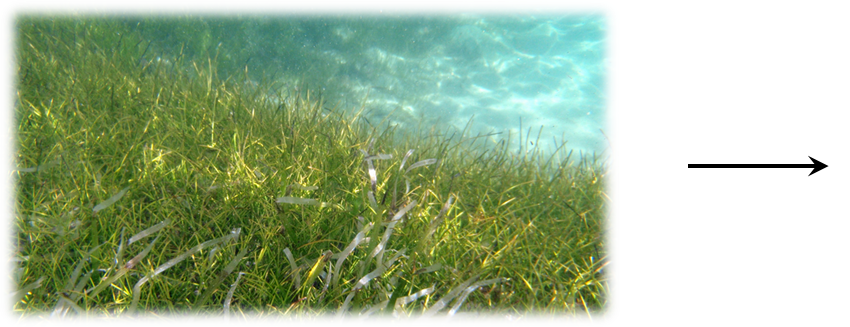
\includegraphics[width=\linewidth]{fig/titlegraphic.png}
\end{minipage}
\begin{minipage}{0.27\linewidth}
\vspace{0.05in}
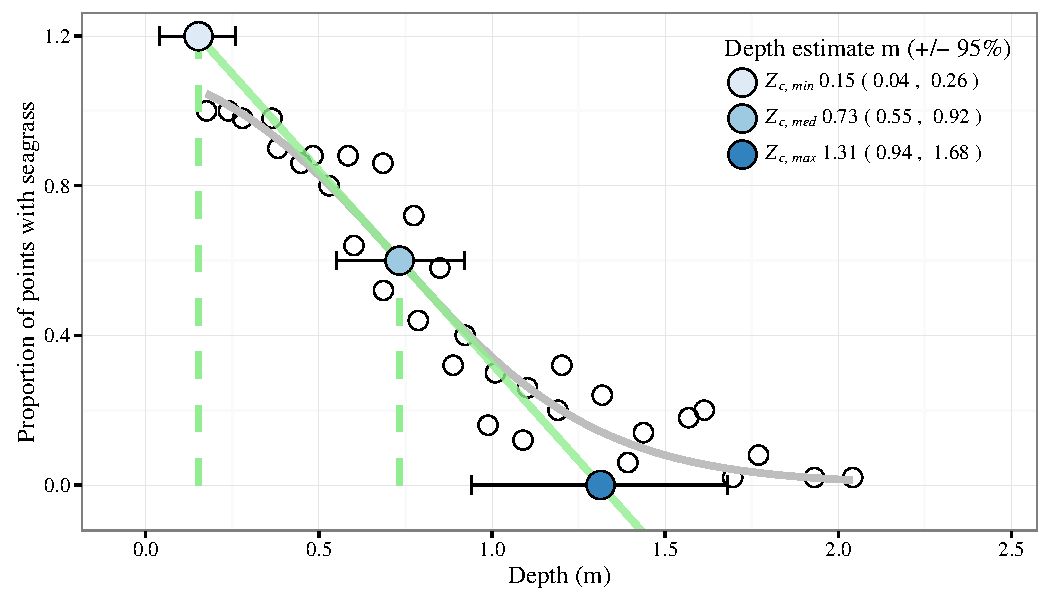
\includegraphics[width=\linewidth]{fig/doc_title.pdf}
\end{minipage}
}

%%%%%%
\begin{frame}[shrink]
\vspace{0.2in}
\titlepage
\end{frame}

\section{Background}

%%%%%%
\begin{frame}{$\vcenter{\hbox{
\includegraphics[width=0.05\paperwidth]{fig/epa_logo.png}}}$\hspace{0.07in}\textbf{Seagrasses and water quality}}
\begin{center}
Seagrasses are beneficial - healthy seagrass, healthy estuary \\~\\
\centerline{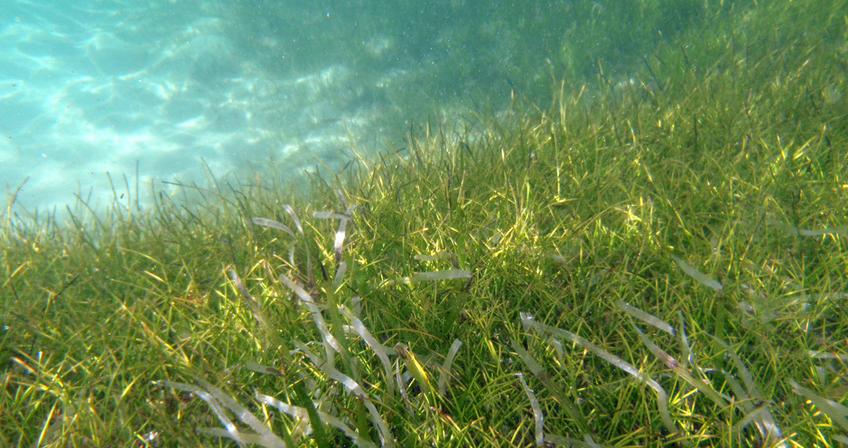
\includegraphics[width = 0.7\textwidth]{fig/sg_pic.png}}
\vspace{0.1in}
Seagrasses are sentinels of water quality \tiny \cite{Short96}
\end{center}
\vfill
\tiny
\hfill \href{https://www.flickr.com/photos/swimvixen2/3581613875/in/photostream/}{flickr.com/photos/swimvixen2}
\end{frame}

%%%%%%
\begin{frame}{$\vcenter{\hbox{
\includegraphics[width=0.05\paperwidth]{fig/epa_logo.png}}}$\hspace{0.07in}\textbf{Seagrasses and water quality}}
\onslide<+->
Nutrient limits using seagrass depth-limit targets \tiny \cite{Steward07}\\~\\
\begin{columns}[T]
\begin{column}{0.45\textwidth}
\centerline{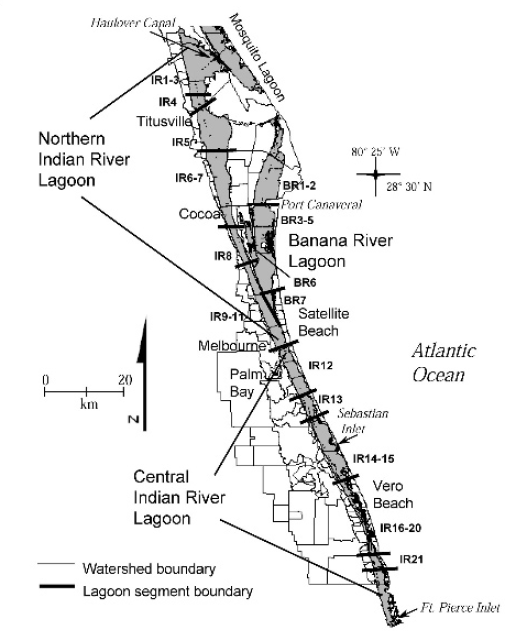
\includegraphics[width = 0.9\textwidth]{fig/irl_map.png}}
\end{column}
\begin{column}{0.45\textwidth}
\centerline{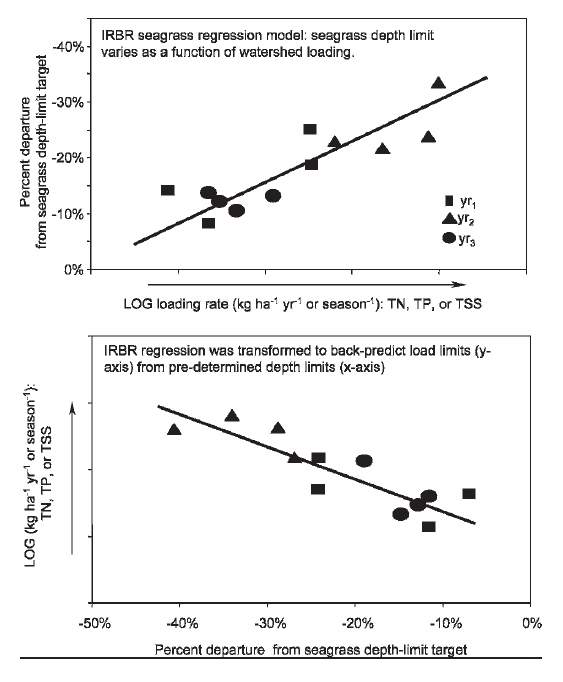
\includegraphics[width = 0.92\textwidth]{fig/irl_reg.png}}
\end{column}
\end{columns}
\end{frame}

%%%%%%
\begin{frame}{$\vcenter{\hbox{
\includegraphics[width=0.05\paperwidth]{fig/epa_logo.png}}}$\hspace{0.07in}\textbf{Seagrasses and water quality}}
\onslide<+->
The maximum depth of colonization is a useful proxy of eutrophication \\~\\
Often used as a basis for establishing nutrient criteria \\~\\
\onslide<+->
\emtxt{Problem 1:} No consensus on the best way to measure depth of colonization \\~\\
\emtxt{Problem 2:} Plenty of data are available but standardized techniques have not been developed \\~\\
\onslide<+->
\begin{block}{Study objective}
Develop and apply an algorithm that uses geospatial data to describe relationships between seagrass depth limits, water clarity, and light requirements \scriptsize [Beck, Hagy, Le, in review]
\end{block}
\end{frame}

%%%%%%
\begin{frame}{$\vcenter{\hbox{
\includegraphics[width=0.05\paperwidth]{fig/epa_logo.png}}}$\hspace{0.07in}\textbf{Seagrasses and water quality}}
\onslide<+->
\emtxt{Existing geospatial datasets} - coastal segments, seagrass areal coverage, bathymetry
\begin{columns}[T]
\begin{column}{0.5\textwidth}
\begin{knitrout}
\definecolor{shadecolor}{rgb}{0.969, 0.969, 0.969}\color{fgcolor}

{\centering 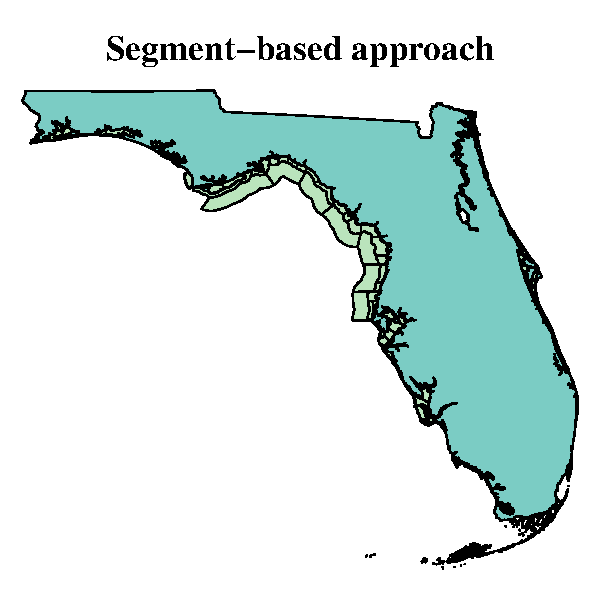
\includegraphics[width=\maxwidth]{fig//segmap-1} 

}



\end{knitrout}
\end{column}
\begin{column}{0.45\textwidth}
\centerline{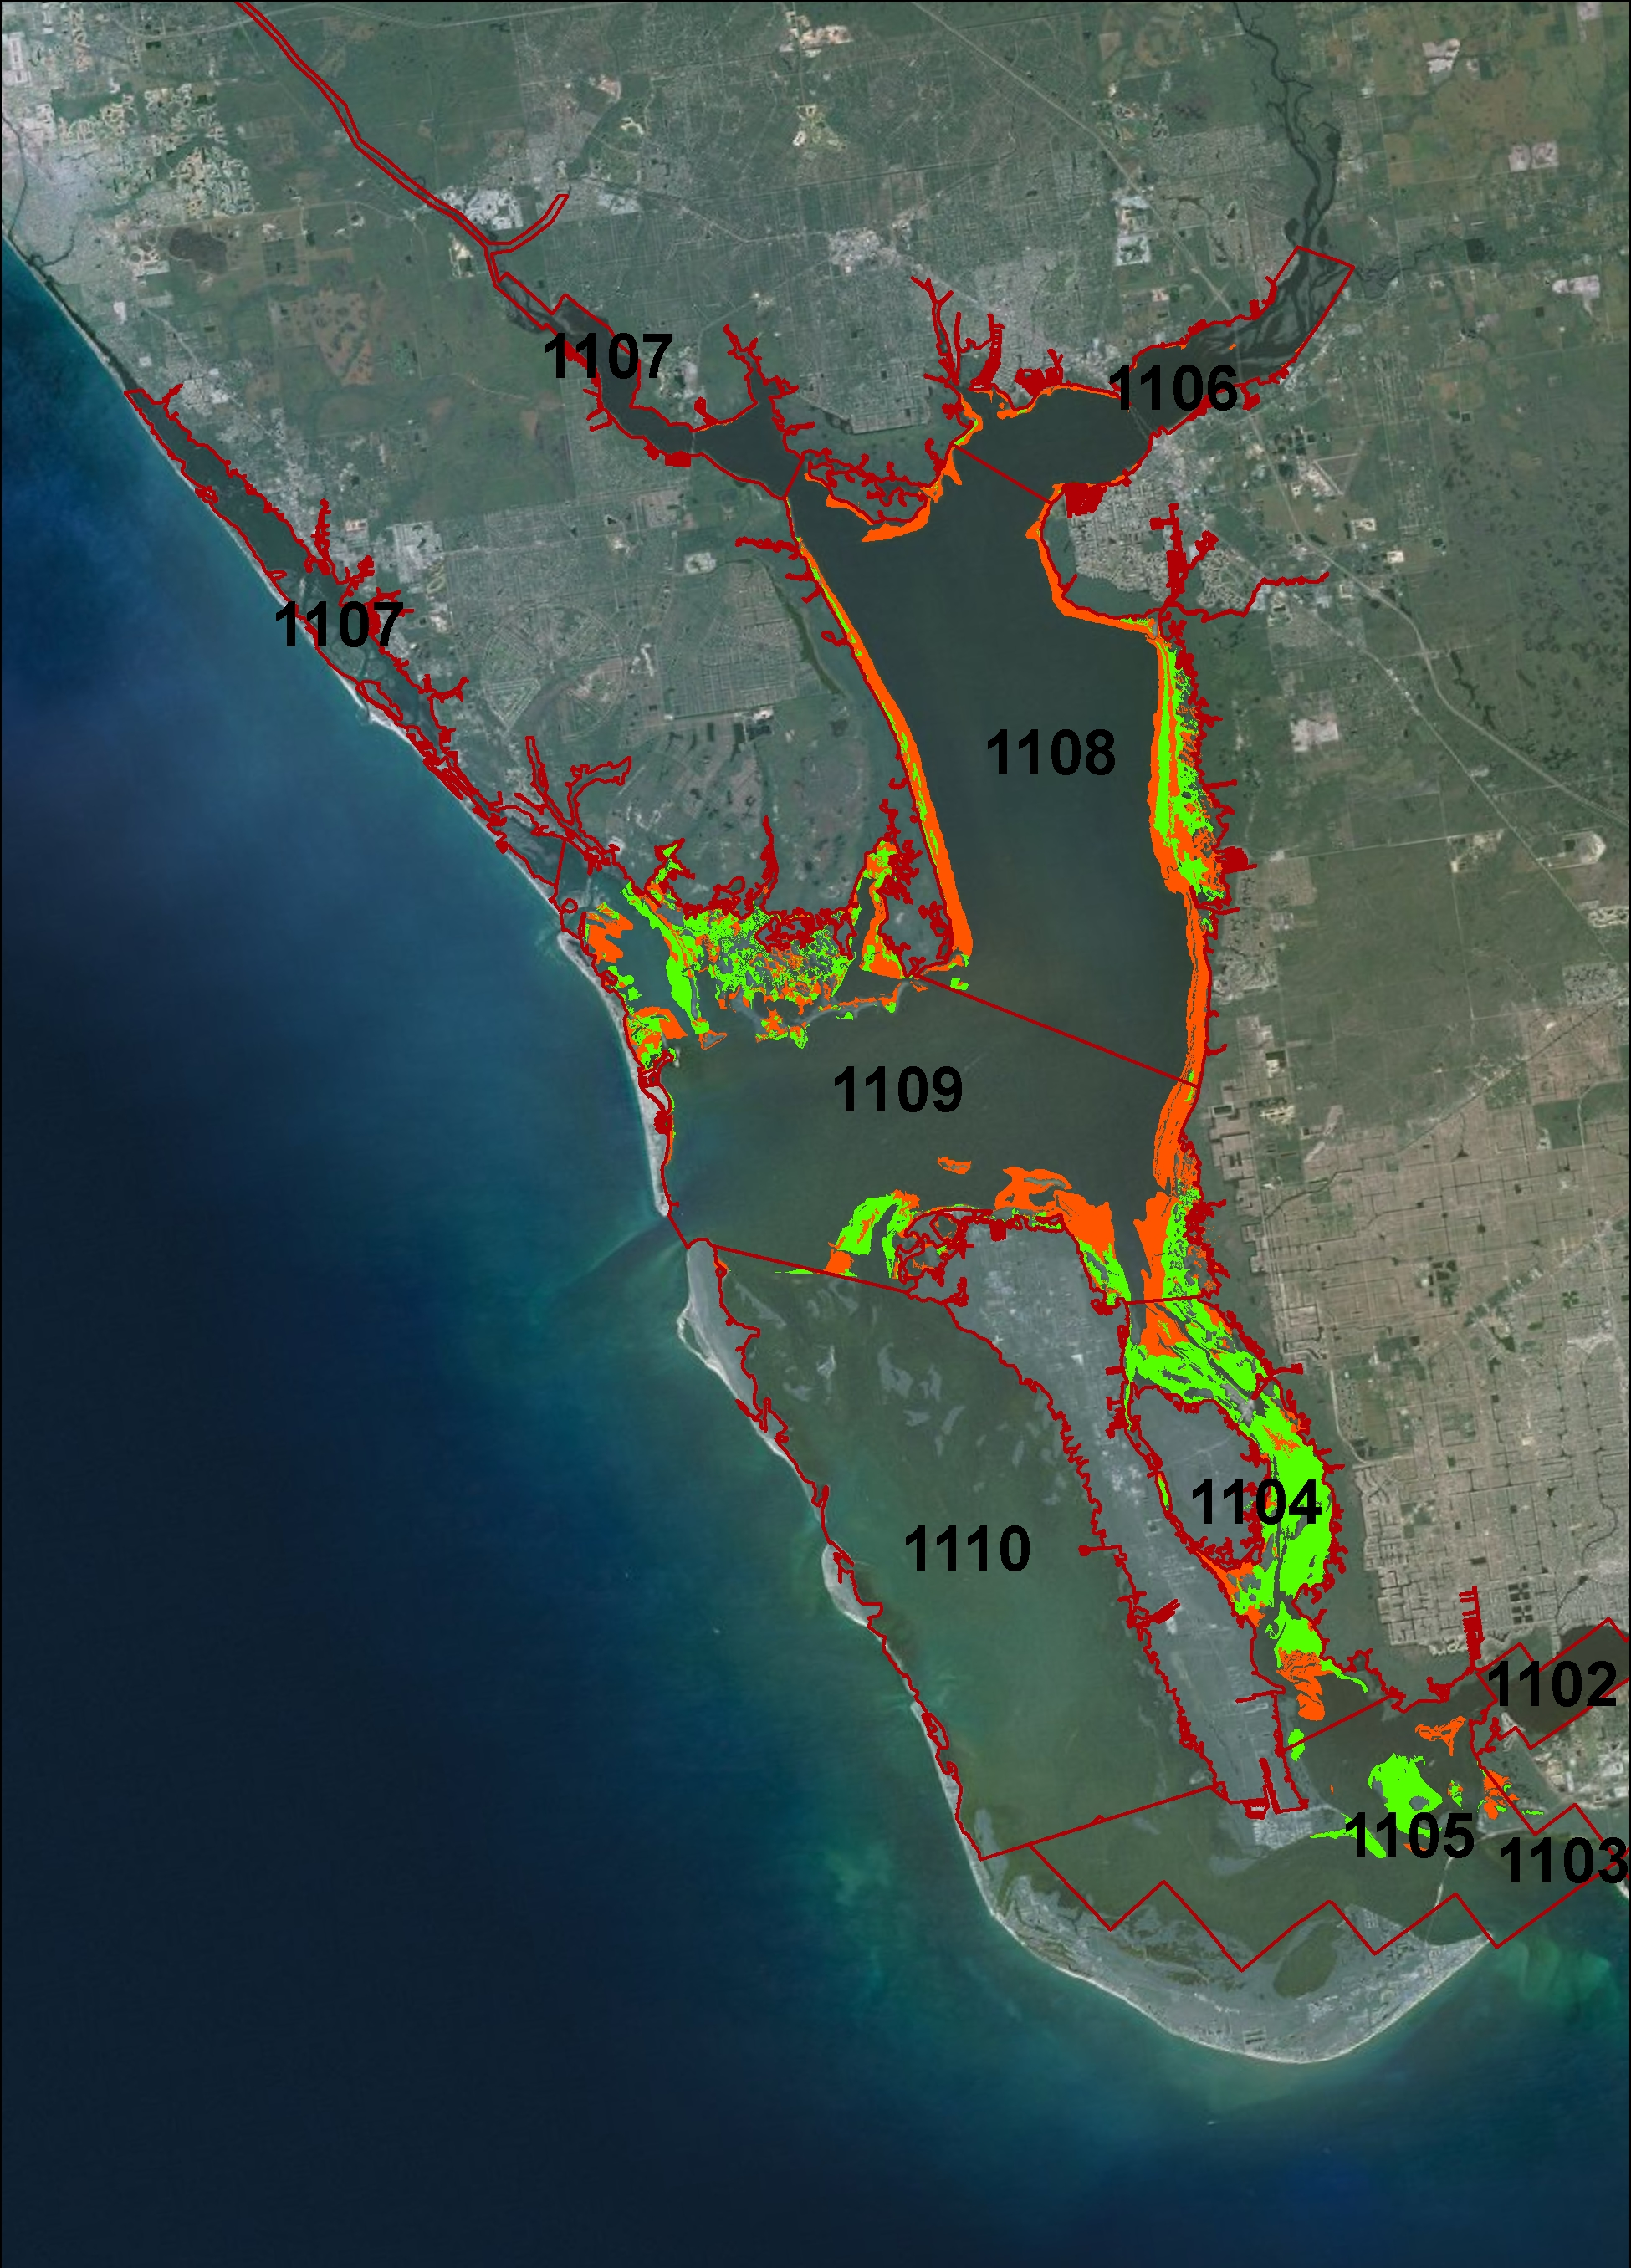
\includegraphics[width = 0.8\textwidth]{fig/Charlotte_Estuary_Segments.jpg}}
\end{column}
\end{columns}
\end{frame}

%%%%%%
\begin{frame}{$\vcenter{\hbox{
\includegraphics[width=0.05\paperwidth]{fig/epa_logo.png}}}$\hspace{0.07in}\textbf{Seagrasses and water quality}}
\onslide<+->
How can we estimate depth of colonization? \\~\\
\begin{columns}[T]
\onslide<+->
\begin{column}{0.32\textwidth}
\emtxt{1.} Pick a segment\\~\\
\centerline{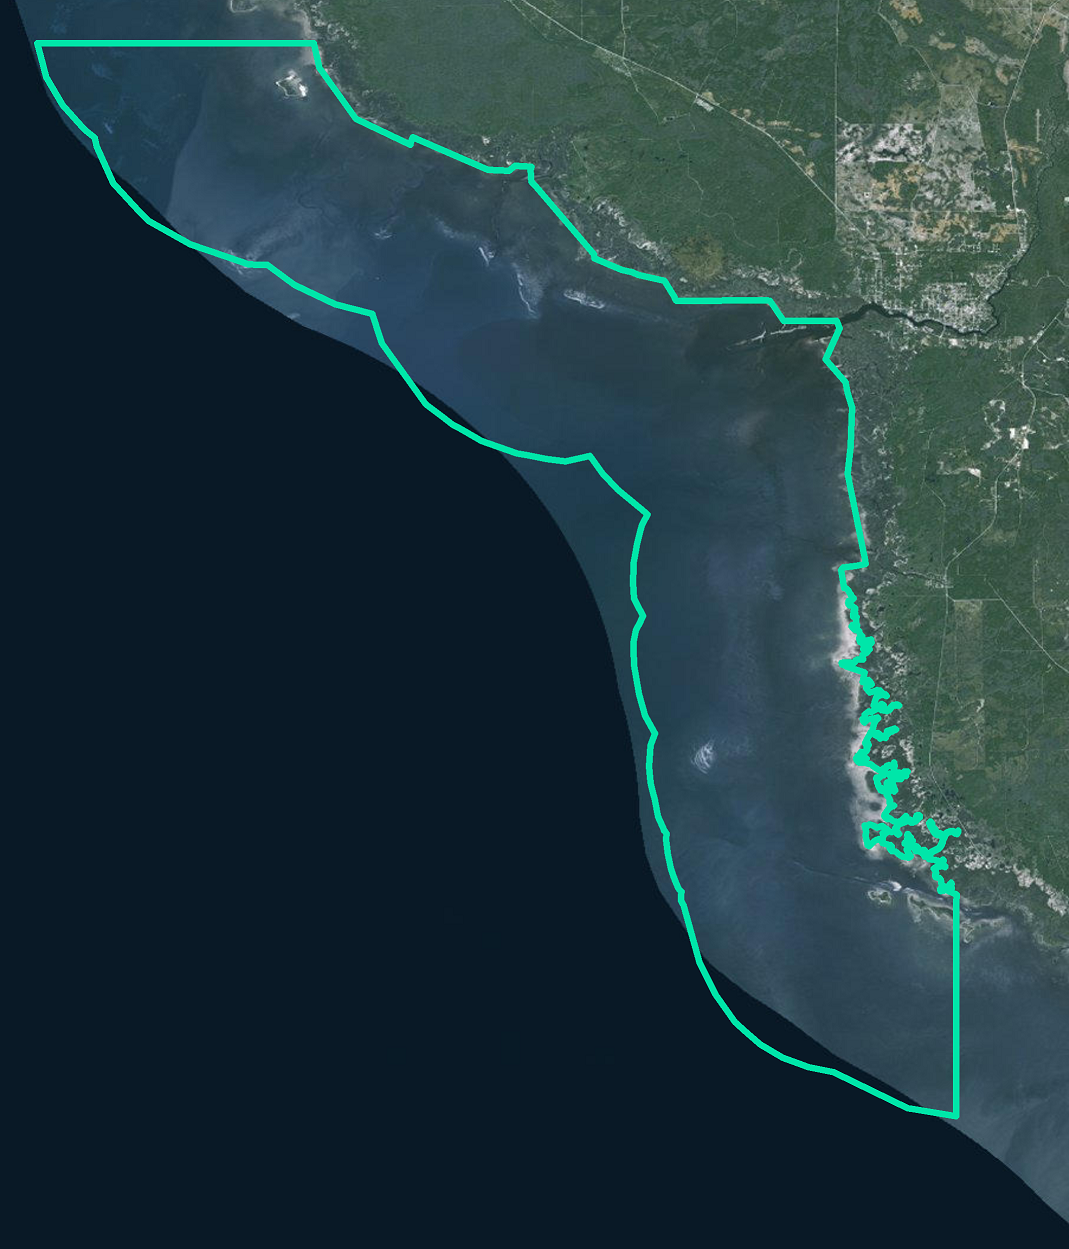
\includegraphics[width = 0.9\textwidth]{fig/map820.png}}
\end{column}
\onslide<+->
\begin{column}{0.32\textwidth}
\emtxt{2.} Get seagrass area \\~\\
\begin{knitrout}
\definecolor{shadecolor}{rgb}{0.969, 0.969, 0.969}\color{fgcolor}

{\centering 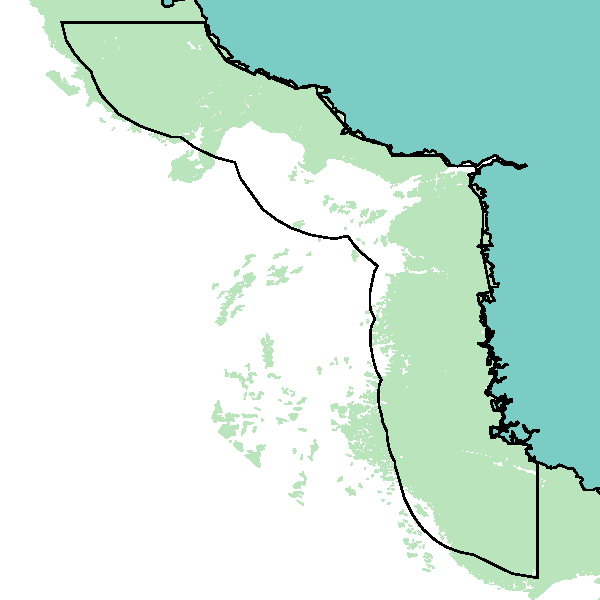
\includegraphics[width=\maxwidth]{fig//segsg-1} 

}



\end{knitrout}
\end{column}
\onslide<+->
\begin{column}{0.32\textwidth}
\emtxt{3.} Get depth points\\~\\
\begin{knitrout}
\definecolor{shadecolor}{rgb}{0.969, 0.969, 0.969}\color{fgcolor}

{\centering 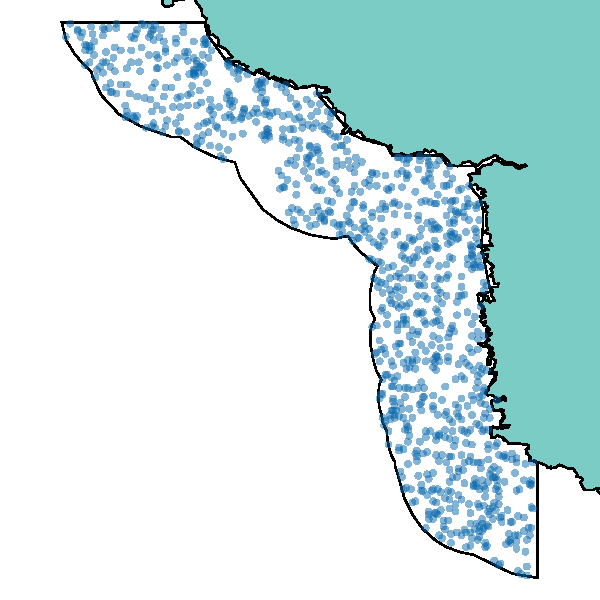
\includegraphics[width=\maxwidth]{fig//segpt-1} 

}



\end{knitrout}
\end{column}
\end{columns}
\vspace{0.15in}
\onslide<+->
\emtxt{4.} Match depth points with p/a of seagrass...
\end{frame}



%%%%%%
\begin{frame}{$\vcenter{\hbox{
\includegraphics[width=0.05\paperwidth]{fig/epa_logo.png}}}$\hspace{0.07in}\textbf{Seagrasses and water quality}}
Plot the distribution of seagrass by increasing depth \\~\\
\includegraphics<1>[width = \textwidth, page = 1]{fig/doc_ex.pdf}
\includegraphics<2>[width = \textwidth, page = 2]{fig/doc_ex.pdf}
\includegraphics<3>[width = \textwidth, page = 3]{fig/doc_ex.pdf}
\end{frame}

%%%%%%
\begin{frame}{$\vcenter{\hbox{
\includegraphics[width=0.05\paperwidth]{fig/epa_logo.png}}}$\hspace{0.07in}\textbf{Seagrasses and water quality}}
\onslide<+->
The estimate depends on the spatial context...
\begin{columns}[T]
\onslide<+->
\begin{column}{0.45\textwidth}
\begin{knitrout}
\definecolor{shadecolor}{rgb}{0.969, 0.969, 0.969}\color{fgcolor}

{\centering 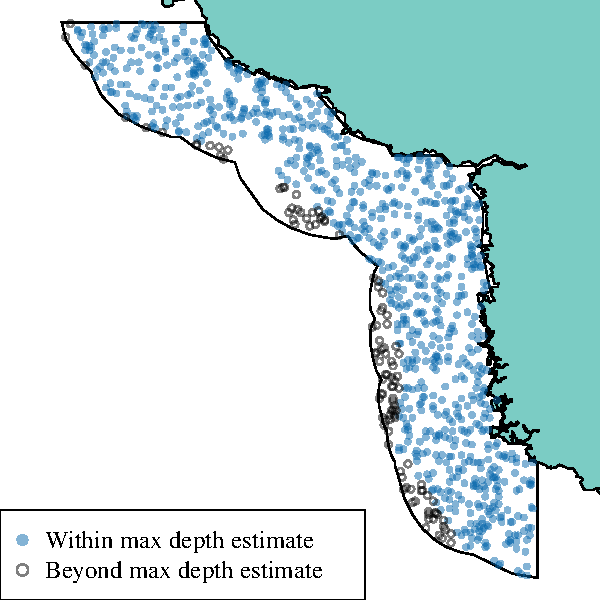
\includegraphics[width=\maxwidth]{fig//docfail1-1} 

}



\end{knitrout}
\end{column}
\onslide<+->
\begin{column}{0.45\textwidth}
\begin{knitrout}
\definecolor{shadecolor}{rgb}{0.969, 0.969, 0.969}\color{fgcolor}

{\centering 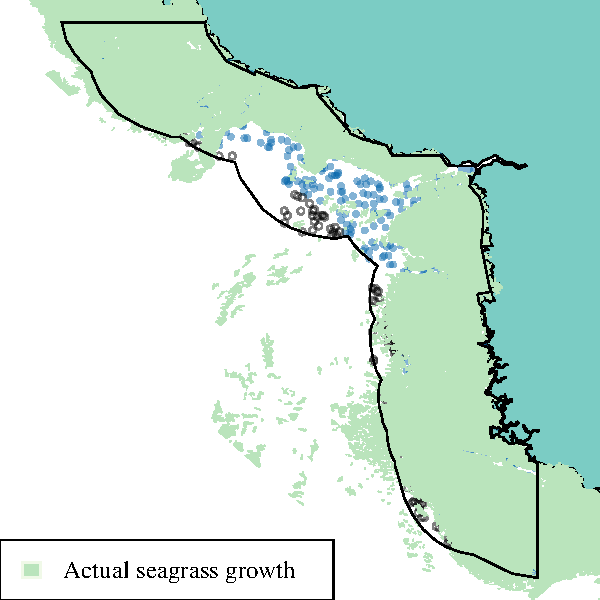
\includegraphics[width=\maxwidth]{fig//docfail2-1} 

}



\end{knitrout}
\end{column}
\end{columns}
\end{frame}


%%%%%%
\begin{frame}{$\vcenter{\hbox{
\includegraphics[width=0.05\paperwidth]{fig/epa_logo.png}}}$\hspace{0.07in}\textbf{Seagrasses and water quality}}
The estimate depends on the spatial context...
\begin{center}
\animategraphics[controls,width=\linewidth,trim = 15mm 2mm 0mm 0mm]{6}{fig/radred}{}{} %frame rate is 12 per/sec
\end{center}
\end{frame}



%%%%%%
\begin{frame}{$\vcenter{\hbox{
\includegraphics[width=0.05\paperwidth]{fig/epa_logo.png}}}$\hspace{0.07in}\textbf{Seagrasses and water quality}}
The estimate depends on the spatial context...
\begin{center}
\animategraphics[controls,width=0.95\linewidth]{6}{fig/radred2}{}{} %frame rate is 12 per/sec
\end{center}
\end{frame}

%%%%%%
\begin{frame}{$\vcenter{\hbox{
\includegraphics[width=0.05\paperwidth]{fig/epa_logo.png}}}$\hspace{0.07in}\textbf{Seagrasses and water quality}}
Applied to four coastal segments
\end{frame}

%%%%%%
\begin{frame}{$\vcenter{\hbox{
\includegraphics[width=0.05\paperwidth]{fig/epa_logo.png}}}$\hspace{0.07in}\textbf{Seagrasses and water quality}}
Can we link depth estimates with water clarity to understand light requirements? 
$\%SI = 100 \cdot \frac{I_{z}}{I_{o}} = exp\left(-K_d \cdot Z_{c,med}\right)$
\end{frame}

% %%%%%%
\begin{frame}{\textbf{Case 2: Seagrass and water quality}}{\textbf{Making the most of existing data}}
\onslide<+->
Benefits of the approach: \\~\\
\begin{itemize}
\item The spatial unit for any estimate of seagrass growth limit is problem-specific \\~\\
\item Allows for a `compliance-point' approach (saves time/money) \\~\\
\item Increased understanding of seagrass growth patterns - natural and anthropogenic drivers \\~\\
\end{itemize}
\onslide<+->
Lots to be done...
\end{frame}

% %%%%%%
% \begin{frame}{\textbf{Case 2: Seagrass and water quality}}{\textbf{Making the most of existing data}}
% Development widget online: \href{https://beckmw.shinyapps.io/sg_depth/}{https://beckmw.shinyapps.io/sg\_depth/}
% \centerline{\includegraphics[width = 0.75\textwidth]{fig/widget.png}}
% \end{frame}
% 
% %%%%%%
% \begin{frame}
% Acknowledgments and contact info:\\~\\
% \begin{columns}
% \begin{column}{0.9\textwidth}
% {\footnotesize
% Research staff and employees at USEPA Gulf Ecology Division, San Francisco Estuary Institute \\~\\
% David Senn, Phil Bresnahan, Emily Novick, James D. Hagy III, Thomas Jabusch
% }
% \end{column}
% \end{columns}
% \vfill
% \begin{columns}
% \begin{column}{0.5\textwidth}
% \begin{center}
% 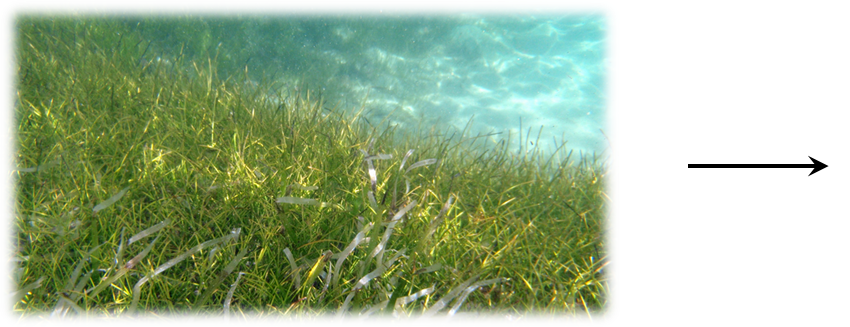
\includegraphics[width=0.7\linewidth]{fig/titlegraphic.png}
% \end{center}
% \end{column}
% \begin{column}{0.5\textwidth}
% \scriptsize
% \begin{center}
% \href{mailto:beck.marcus@epa.gov}{beck.marcus@epa.gov} \\~\\
% Github @fawda123 \\~\\
% Phone: 8509342480
% \end{center}
% \end{column}
% \end{columns}
% \vfill
% Links:\\~\\
% \begin{columns}
% \begin{column}{0.9\textwidth}
% \scriptsize
% This presentation: \href{https://github.com/fawda123/sfei_pres}{\url{https://github.com/fawda123/sfei\_pres}}
% 
% Shiny app: \href{https://beckmw.shinyapps.io/sf_trends/}{\url{https://beckmw.shinyapps.io/sf_trends/}}
% 
% Detailed results: \href{http://fawda123.github.io/sf_trends/README}{\url{http://fawda123.github.io/sf\_trends/README}}
% \end{column}
% \end{columns}
% \end{frame}

%%%%%%
\section{References}
\begin{frame}[t]{\textbf{References}}
\tiny
\setbeamertemplate{bibliography item}{}
\bibliographystyle{apalike_mine}
\bibliography{refs}
\end{frame}

\end{document}
